%a4paper size
\documentclass[a4paper, 12pt]{article}

\usepackage[margin=1in]{geometry}         % for margin
\usepackage{graphicx}                     % for images
\usepackage[toc,page]{appendix}
\usepackage{fancyhdr}                     %for page number in bottom right
\usepackage{listings}                     % for code blocks
\usepackage{color}                        % for colored code blocks ;)
\usepackage{fixltx2e}                     % for text subscripts
\usepackage[T1]{fontenc}                  % ensures < appear correctly
\usepackage{lmodern}                      % same as above
\usepackage{float}                        % makes figures STAY
\usepackage{minted}                       % used for reading code from file
\usepackage{url}                          % for urls in bibi

\graphicspath{{images/}}

\setlength{\parindent}{0pt}

% code block rules

\definecolor{dkgreen}{rgb}{0,0.6,0}
\definecolor{gray}{rgb}{0.5,0.5,0.5}
\definecolor{mauve}{rgb}{0.58,0,0.82}

\lstset{frame=tb,
  language=python,
  aboveskip=3mm,
  belowskip=3mm,
  showstringspaces=false,
  columns=flexible,
  basicstyle={\small\ttfamily},
  numbers=left,
  numberstyle=\tiny\color{gray},
  keywordstyle=\color{blue},
  commentstyle=\color{dkgreen},
  stringstyle=\color{mauve},
  breaklines=true,
  breakatwhitespace=true,
  tabsize=3
}

%TITLE n such
\title{Real-Time Systems in Video Games}
\author{Joshua Siems}
\date{\today}

%Page numbering in bottom right
\pagestyle{fancy}
%clear header and footer
\fancyhead{}
\fancyfoot{}
%get rid of annoying horizontal line
\renewcommand{\headrulewidth}{0pt}
%do what i HWANT
\fancyfoot[R]{\thepage}

%BEGIN DOCUMENT
\begin{document}

\pagenumbering{gobble}

\maketitle

\pagenumbering{arabic}

\section{Introduction}
    A real-time system is a system that must perform specified tasks within a well-defined time constraint. For example, a microcontroller which must read inputs and produce outputs based on the inputs within a certain amount of time would be known as a real-time system. Another kind of real-time system is a video game. Video games would fall under the soft real-time system category. This means that, unlike a hard real-time system, where a missed deadline results in a fatal error, a soft-real time system still cares about the result of an operation even if the deadline is missed. This paper will discuss how video games are soft real-time systems, and will layout a plan for developing a new kind of priority based task execution feature for video games. 

\section{Literature Review}

    \subsection{Video Games as Real-Time Systems}
         The most basic video game must process user inputs, update game variables and update the screen. This must all be completed in a very short amount of time in order to produce the illusion of movement to the user. See Figure \ref{update_cycle} for a simple example of a game loop.
         \\

        \begin{figure}[H]
            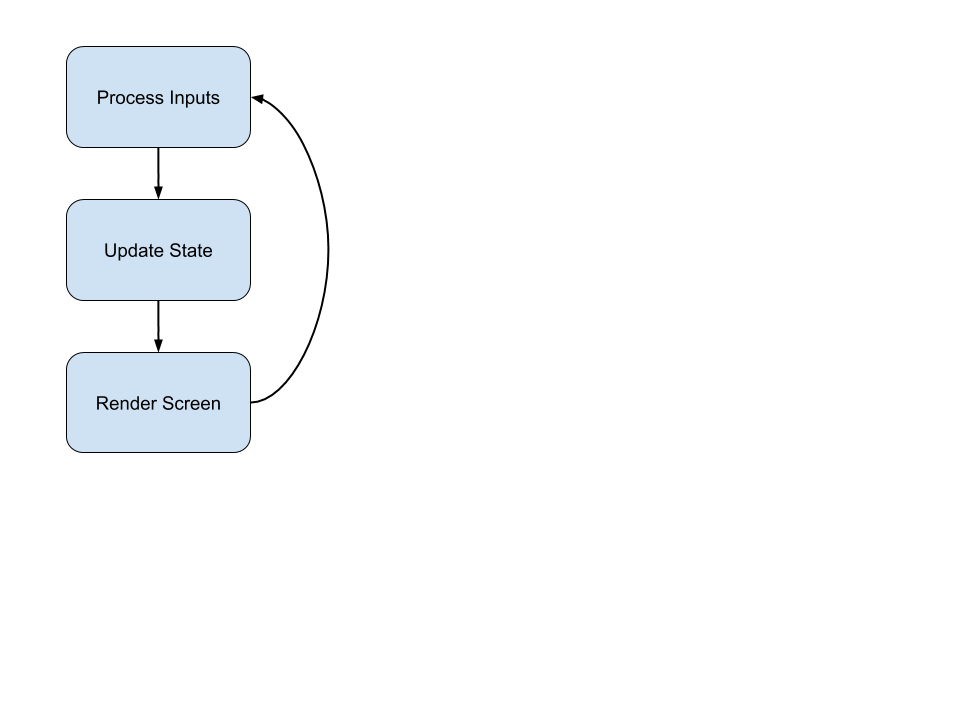
\includegraphics[width=4cm]{game_loop_simple.png}
            \centering
            \caption{Simple game loop.}
            \label{update_cycle}
        \end{figure}

        In order to create this illusion of movement, the game must meet a target frame rate. In the movie world, the industry standard is 24 frames per second. For video games, the targets are much higher. Most games aim to produce at least thirty frames per second, with many more games targeting sixty frames per second. Some video games are even building in support for even higher frame rates that will allow users to play games on 120Hz or 140Hz monitors. \\

        In this sense, a video game can be thought of as a soft real-time system. A soft real-time system is a real-time system where meeting the deadline is desired, but not required. The consequences for missing the deadline in a soft real-time system are miniscule compared to the consequences for missing the deadline in a hard real-time system. For video games, this could be seen as missing the target frame rate for a few frames. The goal is to keep the frame rate close enough to the target so that the user never notices a performance dip. For example, if a game runs at 28 FPS rather than 30 FPS for a few seconds, the user may not even notice. But if a game runs at 15 FPS even for one second, the user will notice the strange delay and the illusion of movement will be ruined. Even then, the game is still playable, and most likely still enjoyable. A video game missing it's deadline is not catastrophic for the user experience, but too many missed deadlines and the player may start to notice. \\

    \subsection{Current Video Game Technology}

        Different video games have different requirements when it comes to the game engine being run. A text based adventure game is perhaps the most simple example, requiring almost no deadlines whatsoever. A text based adventure game will need to read player inputs, and display text to the console. See Figure \ref{text_based_loop}.
        \\

        \begin{figure}[H]
            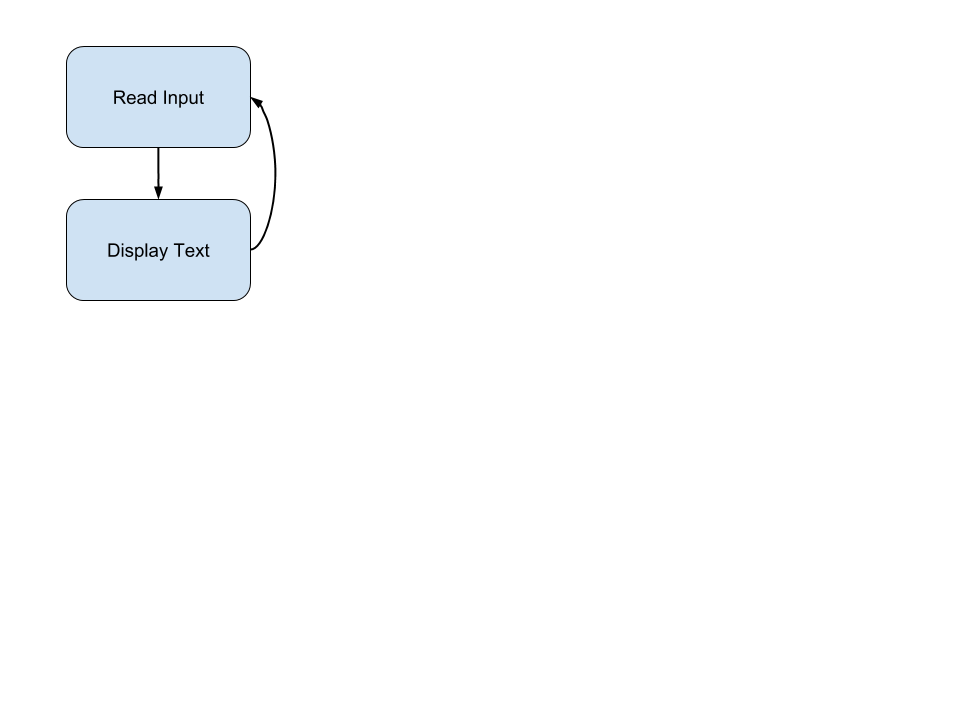
\includegraphics[width=4cm]{text_based_loop.png}
            \centering
            \caption{Text based game loop.}
            \label{text_based_loop}
        \end{figure}

        On the opposite end of the spectrum, a first person shooter may require a much more complex game engine, having to render a 3D world with a sound engine, lighting engine, physics engine, and networking that allows multiple players to play in the same space. All of these components working together creates a very complicated game loop that must fulfill many deadlines. See Figure \ref{fps_game_loop}.

        \begin{figure}[H]
            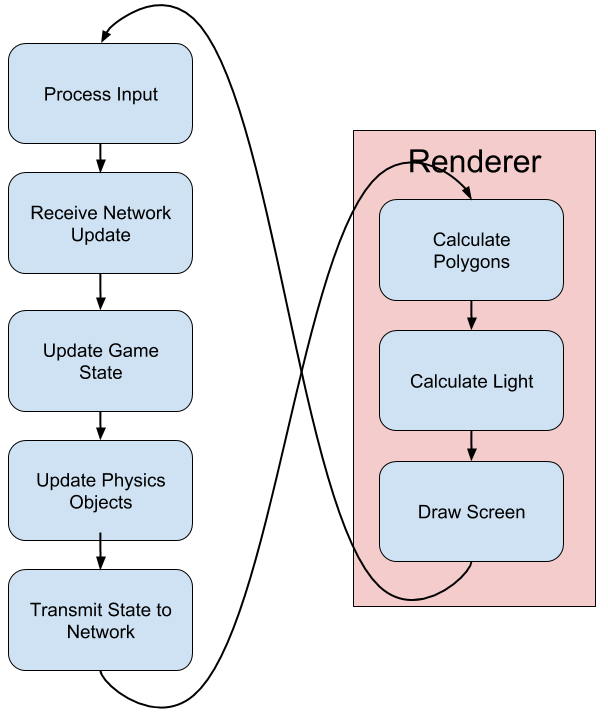
\includegraphics[width=5cm]{fps_loop.png}
            \centering
            \caption{First person shooter game loop.}
            \label{fps_game_loop}
        \end{figure}

        In order to improve performance, many video games split tasks between many processors. For example, a game engine may split out the rendering task into a process on it's own, and compute all other tasks in a separate thread. This will improve performance because at the same time as objects are being drawn to the screen, the physics engine can update and calculate the next locations for those objects. See Figure \ref{multithread_loop}.

        \begin{figure}[H]
            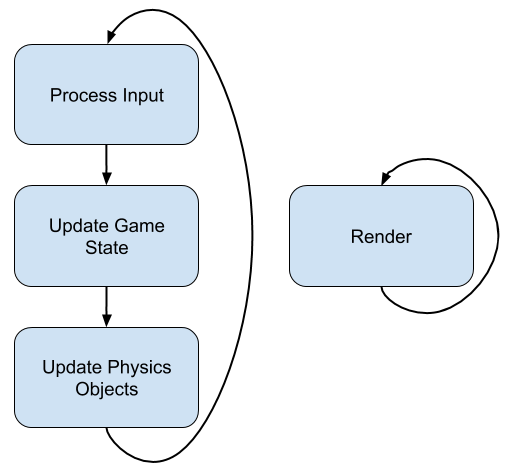
\includegraphics[width=5cm]{multithread_loop.png}
            \centering
            \caption{Multithreaded game loop.}
            \label{multithread_loop}
        \end{figure}



\section{Methodology}
    \subsection{Goals}

        The goal of this project is to demonstrate the power of a game engine that allows the programmer to dynamically change priorities of tasks. A simple video game will accompany the engine to allow the scheduler to be tested. Experiments will be run on the simple game to see what differences are observed when changing the priorities of tasks. The results from these experiments will be documented and analyzed to determine the success of the project. \\

    \subsection{Pseudocode}
        For the sake of simplicity, this project will use a more basic game loop model that only runs on a single processor. This project will process user inputs, update state variables, update physics objects, and then render the screen using a 2D renderer. See Figure \ref{my_loop}.

        \begin{figure}[H]
            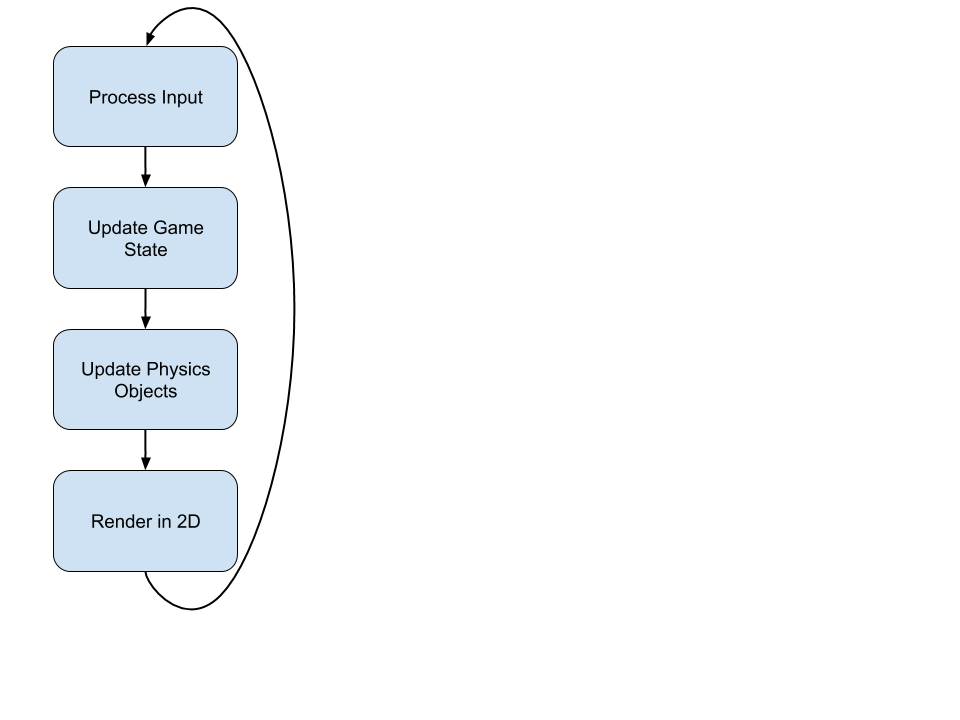
\includegraphics[width=4cm]{my_loop.png}
            \centering
            \caption{Planned game loop for project.}
            \label{my_loop}
        \end{figure}

        The Pseudocode for the program is as follows:

\begin{lstlisting}
main():
    initialize()
    while(playing):
        readInputs()
        updateState()
        updatePhysics()
        drawScreen()

    terminate()
\end{lstlisting}

    \subsection{Scheduler}

        This program will attempt to test a new way of scheduling tasks, one that allows the programmer to change priorities on the fly. The main goal of this scheduler will be to allow the programmer to set priorities of each of the four main loop functions dynamically. For example, if the programmer knows that a certain section requires many physics calculations, he or she can assign the bulk of the run-time to the physics updater. This will in turn reduce the allotted run-time for each of the other processes in the main loop, reducing their accuracy while improving the accuracy of the physics updater.
        \\

        The scheduler will execute the following procedure:
        \begin{enumerate}
            \item{Designate a target frame rate to always meet.}
            \item{Calculate how long each main loop should last based on the given frame rate.}
            \item{Allow the programmer to assign priorities to each process.}
            \item{Allow each process to run for a portion of the loop based on its priority.}
        \end{enumerate}

        For example, if all 4 processes are given a priority of 2, each one would run for 25\% of the time allotted for the main loop. See Figure \ref{even_priority} for an example of this situation. 
        
        \begin{figure}[H]
            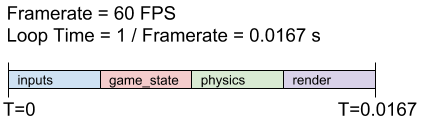
\includegraphics[width=8cm]{even_priority.png}
            \centering
            \caption{Processing distribution with even priority.}
            \label{even_priority}
        \end{figure}

        If updatePhysics() is given a priority of 4, and the others are all 2, updatePhysics() will run for 40\% of the loop while each other function will only run for 20\%. See Figure \ref{phys_priority} for an example of this.

        \begin{figure}[H]
            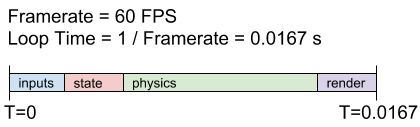
\includegraphics[width=8cm]{phys_priority.png}
            \centering
            \caption{Processing distribution that favors physics calculations}
            \label{phys_priority}
        \end{figure}

\section{Conclusion}
    Video Games are some of the most complicated real-time systems ever created. They must be able to process large amounts of data and produce an output for the user within a short period of time. This project will investigate the effects of allowing the programmer to dynamically change priorities of tasks on the fly. This project will show that given the power, the programmer can improve the gaming experience by allocating resources to specific areas at different times during the game.


\newpage

% REFERENCES
\section{References}

    \begin{thebibliography}{9}
        \bibitem{sim_env}
            M. Joselli, \textit{A Distributed Architecture for Simulation Environments Based on Game Engine Systems}, 2014. [Online]. Available: \url{https://www.springer.com/cda/content/document/cda_downloaddocument/9783642551307-c2.pdf?SGWID=0-0-45-1463314-p176712314}. [Accessed: 28-Feb-2019].
        \bibitem{rt_gl}
            L. Valente, \textit{Real Time Game Loop Models for Single-Player Computer Games}, 2005. [Online]. Available: \url{https://pdfs.semanticscholar.org/f401/4a0328b383ee509ed837ff16af96af1168eb.pdf}. [Accessed: 05-March-2019].
        \bibitem{lb_sch}
            S. Reinalter, \textit{Building a load-balanced task scheduler}, 2012. [Online]. Available: \url{https://blog.molecular-matters.com/2012/04/05/building-a-load-balanced-task-scheduler-part-1-basics/}. [Accessed: 05-March-2019].
        \bibitem{grandmaster}
            \textit{Game Engine part 4}, 2014. [Online]. Available: \url{http://www.grandmaster.nu/blog/?page_id=261}. [Accessed: 05-March-2019].
        \bibitem{gamasutra}
            J. Muffat-Meridol, \textit{Do-it-yourself Game Task Scheduling}, 2010. [Online]. Available: \url{https://www.gamasutra.com/view/feature/132675/sponsored_feature_doityourself_.php}. [Accessed: 05-March-2019].
        \bibitem{}
            D. Binks, \textit{Implementing a Lightweight Task Scheduler}, 2015. [Online]. Available: \url{https://www.enkisoftware.com/devlogpost-20150822-1-Implementing-a-lightweight-task-scheduler}. [Accessed: 05-March-2019].
        \bibitem{}
            \textit{Game Loop}, n.d. [Online]. Available: \url{http://gameprogrammingpatterns.com/game-loop.html}. [Accessed: 05-March-2019].
        \bibitem{}
            P. Dickinson, \textit{Instant Replay: Building a Game Engine with Reproducible Behavior}, 2001. [Online]. Available: \url{http://www.gamasutra.com/view/feature/3057/instant_replay_building_a_game_php}. [Accessed: 05-March-2019].
        \bibitem{}
            K. Witters, \textit{deWiTTERS Game Loop}, 2009. [Online]. Available: \url{http://www.koonsolo.com/news/dewitters-gameloop/}. [Accessed: 05-March-2019].
        \bibitem{}
            R. Monteiro, \textit{Understanding the Game Main Loop}, 2010. [Online]. Available: \url{http://higherorderfun.com/blog/2010/08/17/understanding-the-game-main-loop/}. [Accessed: 05-March-2019].
    \end{thebibliography}

\newpage

%\begin{appendices}

%\section{main.c}
%    \inputminted{c}{../main.c}

%\end{appendices}

\end{document}







